\documentclass[1p]{elsarticle_modified}
%\bibliographystyle{elsarticle-num}

%\usepackage[colorlinks]{hyperref}
%\usepackage{abbrmath_seonhwa} %\Abb, \Ascr, \Acal ,\Abf, \Afrak
\usepackage{amsfonts}
\usepackage{amssymb}
\usepackage{amsmath}
\usepackage{amsthm}
\usepackage{scalefnt}
\usepackage{amsbsy}
\usepackage{kotex}
\usepackage{caption}
\usepackage{subfig}
\usepackage{color}
\usepackage{graphicx}
\usepackage{xcolor} %% white, black, red, green, blue, cyan, magenta, yellow
\usepackage{float}
\usepackage{setspace}
\usepackage{hyperref}

\usepackage{tikz}
\usetikzlibrary{arrows}

\usepackage{multirow}
\usepackage{array} % fixed length table
\usepackage{hhline}

%%%%%%%%%%%%%%%%%%%%%
\makeatletter
\renewcommand*\env@matrix[1][\arraystretch]{%
	\edef\arraystretch{#1}%
	\hskip -\arraycolsep
	\let\@ifnextchar\new@ifnextchar
	\array{*\c@MaxMatrixCols c}}
\makeatother %https://tex.stackexchange.com/questions/14071/how-can-i-increase-the-line-spacing-in-a-matrix
%%%%%%%%%%%%%%%

\usepackage[normalem]{ulem}

\newcommand{\msout}[1]{\ifmmode\text{\sout{\ensuremath{#1}}}\else\sout{#1}\fi}
%SOURCE: \msout is \stkout macro in https://tex.stackexchange.com/questions/20609/strikeout-in-math-mode

\newcommand{\cancel}[1]{
	\ifmmode
	{\color{red}\msout{#1}}
	\else
	{\color{red}\sout{#1}}
	\fi
}

\newcommand{\add}[1]{
	{\color{blue}\uwave{#1}}
}

\newcommand{\replace}[2]{
	\ifmmode
	{\color{red}\msout{#1}}{\color{blue}\uwave{#2}}
	\else
	{\color{red}\sout{#1}}{\color{blue}\uwave{#2}}
	\fi
}

\newcommand{\Sol}{\mathcal{S}} %segment
\newcommand{\D}{D} %diagram
\newcommand{\A}{\mathcal{A}} %arc


%%%%%%%%%%%%%%%%%%%%%%%%%%%%%5 test

\def\sl{\operatorname{\textup{SL}}(2,\Cbb)}
\def\psl{\operatorname{\textup{PSL}}(2,\Cbb)}
\def\quan{\mkern 1mu \triangleright \mkern 1mu}

\theoremstyle{definition}
\newtheorem{thm}{Theorem}[section]
\newtheorem{prop}[thm]{Proposition}
\newtheorem{lem}[thm]{Lemma}
\newtheorem{ques}[thm]{Question}
\newtheorem{cor}[thm]{Corollary}
\newtheorem{defn}[thm]{Definition}
\newtheorem{exam}[thm]{Example}
\newtheorem{rmk}[thm]{Remark}
\newtheorem{alg}[thm]{Algorithm}

\newcommand{\I}{\sqrt{-1}}
\begin{document}

%\begin{frontmatter}
%
%\title{Boundary parabolic representations of knots up to 8 crossings}
%
%%% Group authors per affiliation:
%\author{Yunhi Cho} 
%\address{Department of Mathematics, University of Seoul, Seoul, Korea}
%\ead{yhcho@uos.ac.kr}
%
%
%\author{Seonhwa Kim} %\fnref{s_kim}}
%\address{Center for Geometry and Physics, Institute for Basic Science, Pohang, 37673, Korea}
%\ead{ryeona17@ibs.re.kr}
%
%\author{Hyuk Kim}
%\address{Department of Mathematical Sciences, Seoul National University, Seoul 08826, Korea}
%\ead{hyukkim@snu.ac.kr}
%
%\author{Seokbeom Yoon}
%\address{Department of Mathematical Sciences, Seoul National University, Seoul, 08826,  Korea}
%\ead{sbyoon15@snu.ac.kr}
%
%\begin{abstract}
%We find all boundary parabolic representation of knots up to 8 crossings.
%
%\end{abstract}
%\begin{keyword}
%    \MSC[2010] 57M25 
%\end{keyword}
%
%\end{frontmatter}

%\linenumbers
%\tableofcontents
%
\newcommand\colored[1]{\textcolor{white}{\rule[-0.35ex]{0.8em}{1.4ex}}\kern-0.8em\color{red} #1}%
%\newcommand\colored[1]{\textcolor{white}{ #1}\kern-2.17ex	\textcolor{white}{ #1}\kern-1.81ex	\textcolor{white}{ #1}\kern-2.15ex\color{red}#1	}

{\Large $\underline{10_{107}~(K10a_{66})}$}

\setlength{\tabcolsep}{10pt}
\renewcommand{\arraystretch}{1.6}
\vspace{1cm}\begin{tabular}{m{100pt}>{\centering\arraybackslash}m{274pt}}
\multirow{5}{120pt}{
	\centering
	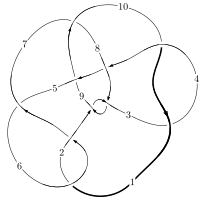
\includegraphics[width=112pt]{../../../GIT/diagram.site/Diagrams/png/191_10_107.png}\\
\ \ \ A knot diagram\footnotemark}&
\allowdisplaybreaks
\textbf{Linearized knot diagam} \\
\cline{2-2}
 &
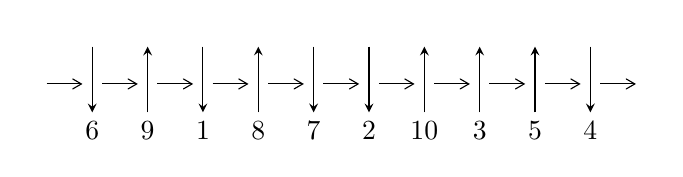
\begin{tikzpicture}[x=20pt, y=17pt]
	% nodes
	\node (C0) at (0, 0) {};
	\node (C1) at (1, 0) {};
	\node (C1U) at (1, +1) {};
	\node (C1D) at (1, -1) {6};

	\node (C2) at (2, 0) {};
	\node (C2U) at (2, +1) {};
	\node (C2D) at (2, -1) {9};

	\node (C3) at (3, 0) {};
	\node (C3U) at (3, +1) {};
	\node (C3D) at (3, -1) {1};

	\node (C4) at (4, 0) {};
	\node (C4U) at (4, +1) {};
	\node (C4D) at (4, -1) {8};

	\node (C5) at (5, 0) {};
	\node (C5U) at (5, +1) {};
	\node (C5D) at (5, -1) {7};

	\node (C6) at (6, 0) {};
	\node (C6U) at (6, +1) {};
	\node (C6D) at (6, -1) {2};

	\node (C7) at (7, 0) {};
	\node (C7U) at (7, +1) {};
	\node (C7D) at (7, -1) {10};

	\node (C8) at (8, 0) {};
	\node (C8U) at (8, +1) {};
	\node (C8D) at (8, -1) {3};

	\node (C9) at (9, 0) {};
	\node (C9U) at (9, +1) {};
	\node (C9D) at (9, -1) {5};

	\node (C10) at (10, 0) {};
	\node (C10U) at (10, +1) {};
	\node (C10D) at (10, -1) {4};
	\node (C11) at (11, 0) {};

	% arrows
	\draw[->,>={angle 60}]
	(C0) edge (C1) (C1) edge (C2) (C2) edge (C3) (C3) edge (C4) (C4) edge (C5) (C5) edge (C6) (C6) edge (C7) (C7) edge (C8) (C8) edge (C9) (C9) edge (C10) (C10) edge (C11) ;	\draw[->,>=stealth]
	(C1U) edge (C1D) (C2D) edge (C2U) (C3U) edge (C3D) (C4D) edge (C4U) (C5U) edge (C5D) (C6U) edge (C6D) (C7D) edge (C7U) (C8D) edge (C8U) (C9D) edge (C9U) (C10U) edge (C10D) ;
	\end{tikzpicture} \\
\hhline{~~} \\& 
\textbf{Solving Sequence} \\ \cline{2-2} 
 &
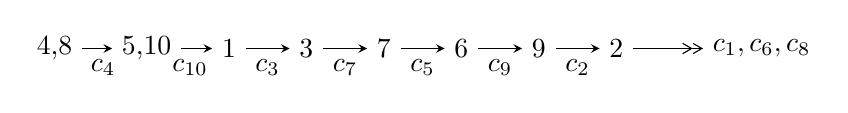
\begin{tikzpicture}[x=28pt, y=7pt]
	% node
	\node (A0) at (-1/8, 0) {4,8};
	\node (A1) at (17/16, 0) {5,10};
	\node (A2) at (17/8, 0) {1};
	\node (A3) at (25/8, 0) {3};
	\node (A4) at (33/8, 0) {7};
	\node (A5) at (41/8, 0) {6};
	\node (A6) at (49/8, 0) {9};
	\node (A7) at (57/8, 0) {2};
	\node (C1) at (1/2, -1) {$c_{4}$};
	\node (C2) at (13/8, -1) {$c_{10}$};
	\node (C3) at (21/8, -1) {$c_{3}$};
	\node (C4) at (29/8, -1) {$c_{7}$};
	\node (C5) at (37/8, -1) {$c_{5}$};
	\node (C6) at (45/8, -1) {$c_{9}$};
	\node (C7) at (53/8, -1) {$c_{2}$};
	\node (A8) at (9, 0) {$c_{1},c_{6},c_{8}$};

	% edge
	\draw[->,>=stealth]	
	(A0) edge (A1) (A1) edge (A2) (A2) edge (A3) (A3) edge (A4) (A4) edge (A5) (A5) edge (A6) (A6) edge (A7) ;
	\draw[->>,>={angle 60}]	
	(A7) edge (A8);
\end{tikzpicture} \\ 

\end{tabular} \\

\footnotetext{
The image of knot diagram is generated by the software ``\textbf{Draw programme}" developed by Andrew Bartholomew(\url{http://www.layer8.co.uk/maths/draw/index.htm\#Running-draw}), where we modified some parts for our purpose(\url{https://github.com/CATsTAILs/LinksPainter}).
}\phantom \\ \newline 
\centering \textbf{Ideals for irreducible components\footnotemark of $X_{\text{par}}$} 
 
\begin{align*}
I^u_{1}&=\langle 
3.47436\times10^{121} u^{53}+1.72858\times10^{122} u^{52}+\cdots+9.59630\times10^{122} b+1.78292\times10^{122},\\
\phantom{I^u_{1}}&\phantom{= \langle  }-1.53764\times10^{122} u^{53}-8.54360\times10^{122} u^{52}+\cdots+9.59630\times10^{122} a-1.60436\times10^{123},\;u^{54}+5 u^{53}+\cdots+u+2\rangle \\
I^u_{2}&=\langle 
u^7- u^6- u^4+b+1,\;u^4+a- u,\;u^8- u^5- u^4+u+1\rangle \\
\\
\end{align*}
\raggedright * 2 irreducible components of $\dim_{\mathbb{C}}=0$, with total 62 representations.\\
\footnotetext{All coefficients of polynomials are rational numbers. But the coefficients are sometimes approximated in decimal forms when there is not enough margin.}
\newpage
\renewcommand{\arraystretch}{1}
\centering \section*{I. $I^u_{1}= \langle 3.47\times10^{121} u^{53}+1.73\times10^{122} u^{52}+\cdots+9.60\times10^{122} b+1.78\times10^{122},\;-1.54\times10^{122} u^{53}-8.54\times10^{122} u^{52}+\cdots+9.60\times10^{122} a-1.60\times10^{123},\;u^{54}+5 u^{53}+\cdots+u+2 \rangle$}
\flushleft \textbf{(i) Arc colorings}\\
\begin{tabular}{m{7pt} m{180pt} m{7pt} m{180pt} }
\flushright $a_{4}=$&$\begin{pmatrix}1\\0\end{pmatrix}$ \\
\flushright $a_{8}=$&$\begin{pmatrix}0\\u\end{pmatrix}$ \\
\flushright $a_{5}=$&$\begin{pmatrix}1\\- u^2\end{pmatrix}$ \\
\flushright $a_{10}=$&$\begin{pmatrix}0.160232 u^{53}+0.890301 u^{52}+\cdots+13.7576 u+1.67185\\-0.0362051 u^{53}-0.180130 u^{52}+\cdots-2.75155 u-0.185792\end{pmatrix}$ \\
\flushright $a_{1}=$&$\begin{pmatrix}0.196437 u^{53}+1.07043 u^{52}+\cdots+16.5092 u+1.85764\\-0.0362051 u^{53}-0.180130 u^{52}+\cdots-2.75155 u-0.185792\end{pmatrix}$ \\
\flushright $a_{3}=$&$\begin{pmatrix}0.0961420 u^{53}+0.569261 u^{52}+\cdots-3.23497 u-4.09449\\0.100644 u^{53}+0.590672 u^{52}+\cdots+0.552368 u+1.22006\end{pmatrix}$ \\
\flushright $a_{7}=$&$\begin{pmatrix}-0.643905 u^{53}-3.03045 u^{52}+\cdots+15.9005 u+4.34106\\0.176005 u^{53}+0.787005 u^{52}+\cdots-3.07121 u-0.393571\end{pmatrix}$ \\
\flushright $a_{6}=$&$\begin{pmatrix}-0.101496 u^{53}-0.690858 u^{52}+\cdots-23.6713 u-4.01578\\-0.0385911 u^{53}-0.220008 u^{52}+\cdots+3.07522 u+0.327925\end{pmatrix}$ \\
\flushright $a_{9}=$&$\begin{pmatrix}0.128037 u^{53}+0.744252 u^{52}+\cdots+16.9188 u+2.03592\\-0.0983217 u^{53}-0.460344 u^{52}+\cdots-2.80102 u-0.155940\end{pmatrix}$ \\
\flushright $a_{2}=$&$\begin{pmatrix}-0.491512 u^{53}-2.79234 u^{52}+\cdots-8.87717 u-1.13816\\0.0534818 u^{53}+0.417725 u^{52}+\cdots+0.472700 u-0.0509315\end{pmatrix}$\\&\end{tabular}
\flushleft \textbf{(ii) Obstruction class $= -1$}\\~\\
\flushleft \textbf{(iii) Cusp Shapes $= 0.461877 u^{53}+2.14757 u^{52}+\cdots-1.68088 u-2.26465$}\\~\\
\newpage\renewcommand{\arraystretch}{1}
\flushleft \textbf{(iv) u-Polynomials at the component}\newline \\
\begin{tabular}{m{50pt}|m{274pt}}
Crossings & \hspace{64pt}u-Polynomials at each crossing \\
\hline $$\begin{aligned}c_{1},c_{6}\end{aligned}$$&$\begin{aligned}
&u^{54}- u^{53}+\cdots-14 u+7
\end{aligned}$\\
\hline $$\begin{aligned}c_{2},c_{8}\end{aligned}$$&$\begin{aligned}
&u^{54}- u^{53}+\cdots+9 u^2+1
\end{aligned}$\\
\hline $$\begin{aligned}c_{3},c_{10}\end{aligned}$$&$\begin{aligned}
&u^{54}-2 u^{53}+\cdots-75 u+19
\end{aligned}$\\
\hline $$\begin{aligned}c_{4}\end{aligned}$$&$\begin{aligned}
&u^{54}+5 u^{53}+\cdots+u+2
\end{aligned}$\\
\hline $$\begin{aligned}c_{5}\end{aligned}$$&$\begin{aligned}
&u^{54}+23 u^{53}+\cdots+406 u+49
\end{aligned}$\\
\hline $$\begin{aligned}c_{7}\end{aligned}$$&$\begin{aligned}
&u^{54}+7 u^{53}+\cdots+123 u+49
\end{aligned}$\\
\hline $$\begin{aligned}c_{9}\end{aligned}$$&$\begin{aligned}
&u^{54}-3 u^{51}+\cdots+19 u+1
\end{aligned}$\\
\hline
\end{tabular}\\~\\
\newpage\renewcommand{\arraystretch}{1}
\flushleft \textbf{(v) Riley Polynomials at the component}\newline \\
\begin{tabular}{m{50pt}|m{274pt}}
Crossings & \hspace{64pt}Riley Polynomials at each crossing \\
\hline $$\begin{aligned}c_{1},c_{6}\end{aligned}$$&$\begin{aligned}
&y^{54}-23 y^{53}+\cdots-406 y+49
\end{aligned}$\\
\hline $$\begin{aligned}c_{2},c_{8}\end{aligned}$$&$\begin{aligned}
&y^{54}+33 y^{53}+\cdots+18 y+1
\end{aligned}$\\
\hline $$\begin{aligned}c_{3},c_{10}\end{aligned}$$&$\begin{aligned}
&y^{54}+36 y^{53}+\cdots+911 y+361
\end{aligned}$\\
\hline $$\begin{aligned}c_{4}\end{aligned}$$&$\begin{aligned}
&y^{54}-3 y^{53}+\cdots+43 y+4
\end{aligned}$\\
\hline $$\begin{aligned}c_{5}\end{aligned}$$&$\begin{aligned}
&y^{54}+21 y^{53}+\cdots+31458 y+2401
\end{aligned}$\\
\hline $$\begin{aligned}c_{7}\end{aligned}$$&$\begin{aligned}
&y^{54}-15 y^{53}+\cdots-60601 y+2401
\end{aligned}$\\
\hline $$\begin{aligned}c_{9}\end{aligned}$$&$\begin{aligned}
&y^{54}+42 y^{52}+\cdots-17 y+1
\end{aligned}$\\
\hline
\end{tabular}\\~\\
\newpage\flushleft \textbf{(vi) Complex Volumes and Cusp Shapes}
$$\begin{array}{c|c|c}  
\text{Solutions to }I^u_{1}& \I (\text{vol} + \sqrt{-1}CS) & \text{Cusp shape}\\
 \hline 
\begin{aligned}
u &= -0.961364 + 0.112432 I \\
a &= -0.572959 - 0.054695 I \\
b &= -0.66278 - 1.34570 I\end{aligned}
 & \phantom{-}2.22290 - 1.39898 I & \phantom{-}4.85913 - 0.38785 I \\ \hline\begin{aligned}
u &= -0.961364 - 0.112432 I \\
a &= -0.572959 + 0.054695 I \\
b &= -0.66278 + 1.34570 I\end{aligned}
 & \phantom{-}2.22290 + 1.39898 I & \phantom{-}4.85913 + 0.38785 I \\ \hline\begin{aligned}
u &= \phantom{-}0.558405 + 0.788615 I \\
a &= -1.055990 + 0.295330 I \\
b &= -1.156370 + 0.001294 I\end{aligned}
 & -1.38784 + 3.43862 I & -1.22590 - 4.16430 I \\ \hline\begin{aligned}
u &= \phantom{-}0.558405 - 0.788615 I \\
a &= -1.055990 - 0.295330 I \\
b &= -1.156370 - 0.001294 I\end{aligned}
 & -1.38784 - 3.43862 I & -1.22590 + 4.16430 I \\ \hline\begin{aligned}
u &= -0.679141 + 0.788921 I \\
a &= \phantom{-}1.121720 + 0.119877 I \\
b &= \phantom{-}1.268940 - 0.162988 I\end{aligned}
 & -3.08313 - 8.79179 I & -2.77233 + 8.25769 I \\ \hline\begin{aligned}
u &= -0.679141 - 0.788921 I \\
a &= \phantom{-}1.121720 - 0.119877 I \\
b &= \phantom{-}1.268940 + 0.162988 I\end{aligned}
 & -3.08313 + 8.79179 I & -2.77233 - 8.25769 I \\ \hline\begin{aligned}
u &= \phantom{-}0.149591 + 1.036280 I \\
a &= \phantom{-}0.578889 + 1.147670 I \\
b &= \phantom{-}0.516207 + 0.654055 I\end{aligned}
 & -2.54046 + 2.78962 I & -3.14255 - 2.96255 I \\ \hline\begin{aligned}
u &= \phantom{-}0.149591 - 1.036280 I \\
a &= \phantom{-}0.578889 - 1.147670 I \\
b &= \phantom{-}0.516207 - 0.654055 I\end{aligned}
 & -2.54046 - 2.78962 I & -3.14255 + 2.96255 I \\ \hline\begin{aligned}
u &= -0.830583 + 0.437641 I \\
a &= -1.154350 + 0.444935 I \\
b &= -0.722840 - 0.321202 I\end{aligned}
 & -0.20915 - 4.60279 I & -0.54557 + 5.84363 I \\ \hline\begin{aligned}
u &= -0.830583 - 0.437641 I \\
a &= -1.154350 - 0.444935 I \\
b &= -0.722840 + 0.321202 I\end{aligned}
 & -0.20915 + 4.60279 I & -0.54557 - 5.84363 I\\
 \hline 
 \end{array}$$\newpage$$\begin{array}{c|c|c}  
\text{Solutions to }I^u_{1}& \I (\text{vol} + \sqrt{-1}CS) & \text{Cusp shape}\\
 \hline 
\begin{aligned}
u &= \phantom{-}1.043990 + 0.201174 I \\
a &= \phantom{-}0.829255 - 0.100464 I \\
b &= \phantom{-}0.82599 - 1.28687 I\end{aligned}
 & \phantom{-}1.65482 + 5.78575 I & \phantom{-}2.51560 - 7.01331 I \\ \hline\begin{aligned}
u &= \phantom{-}1.043990 - 0.201174 I \\
a &= \phantom{-}0.829255 + 0.100464 I \\
b &= \phantom{-}0.82599 + 1.28687 I\end{aligned}
 & \phantom{-}1.65482 - 5.78575 I & \phantom{-}2.51560 + 7.01331 I \\ \hline\begin{aligned}
u &= \phantom{-}0.992623 + 0.381167 I \\
a &= \phantom{-}1.089900 + 0.189030 I \\
b &= \phantom{-}0.831671 - 0.901756 I\end{aligned}
 & \phantom{-}0.562845 + 1.252740 I & -1.233700 + 0.528973 I \\ \hline\begin{aligned}
u &= \phantom{-}0.992623 - 0.381167 I \\
a &= \phantom{-}1.089900 - 0.189030 I \\
b &= \phantom{-}0.831671 + 0.901756 I\end{aligned}
 & \phantom{-}0.562845 - 1.252740 I & -1.233700 - 0.528973 I \\ \hline\begin{aligned}
u &= -0.703334 + 0.548552 I \\
a &= -1.35884 + 0.54589 I \\
b &= -0.486359 - 1.054920 I\end{aligned}
 & \phantom{-}0.47962 - 3.24903 I & -2.21240 + 6.16822 I \\ \hline\begin{aligned}
u &= -0.703334 - 0.548552 I \\
a &= -1.35884 - 0.54589 I \\
b &= -0.486359 + 1.054920 I\end{aligned}
 & \phantom{-}0.47962 + 3.24903 I & -2.21240 - 6.16822 I \\ \hline\begin{aligned}
u &= \phantom{-}0.090692 + 0.846569 I \\
a &= -0.681551 + 0.813861 I \\
b &= -0.628328 + 0.416871 I\end{aligned}
 & -1.44225 + 1.32993 I & -2.25893 - 3.81749 I \\ \hline\begin{aligned}
u &= \phantom{-}0.090692 - 0.846569 I \\
a &= -0.681551 - 0.813861 I \\
b &= -0.628328 - 0.416871 I\end{aligned}
 & -1.44225 - 1.32993 I & -2.25893 + 3.81749 I \\ \hline\begin{aligned}
u &= \phantom{-}0.039167 + 1.215900 I \\
a &= \phantom{-}0.12642 + 1.42966 I \\
b &= \phantom{-}0.116430 + 0.911737 I\end{aligned}
 & -3.14719 - 1.85744 I & \phantom{-0.000000 -}0. + 4.53165 I \\ \hline\begin{aligned}
u &= \phantom{-}0.039167 - 1.215900 I \\
a &= \phantom{-}0.12642 - 1.42966 I \\
b &= \phantom{-}0.116430 - 0.911737 I\end{aligned}
 & -3.14719 + 1.85744 I & \phantom{-0.000000 } 0. - 4.53165 I\\
 \hline 
 \end{array}$$\newpage$$\begin{array}{c|c|c}  
\text{Solutions to }I^u_{1}& \I (\text{vol} + \sqrt{-1}CS) & \text{Cusp shape}\\
 \hline 
\begin{aligned}
u &= -0.599196 + 1.091280 I \\
a &= \phantom{-}0.674349 + 0.091168 I \\
b &= \phantom{-}0.815766 - 0.311304 I\end{aligned}
 & -6.71595 - 1.65367 I & -8.08588 + 0. I\phantom{ +0.000000I} \\ \hline\begin{aligned}
u &= -0.599196 - 1.091280 I \\
a &= \phantom{-}0.674349 - 0.091168 I \\
b &= \phantom{-}0.815766 + 0.311304 I\end{aligned}
 & -6.71595 + 1.65367 I & -8.08588 + 0. I\phantom{ +0.000000I} \\ \hline\begin{aligned}
u &= \phantom{-}0.741079 + 0.137552 I \\
a &= \phantom{-}1.194820 + 0.322038 I \\
b &= \phantom{-}0.296885 - 0.144859 I\end{aligned}
 & \phantom{-}1.46648 + 0.54178 I & \phantom{-}5.93628 - 0.17488 I \\ \hline\begin{aligned}
u &= \phantom{-}0.741079 - 0.137552 I \\
a &= \phantom{-}1.194820 - 0.322038 I \\
b &= \phantom{-}0.296885 + 0.144859 I\end{aligned}
 & \phantom{-}1.46648 - 0.54178 I & \phantom{-}5.93628 + 0.17488 I \\ \hline\begin{aligned}
u &= -0.452082 + 0.566184 I \\
a &= \phantom{-}0.536326 + 0.764262 I \\
b &= \phantom{-}0.02633 + 1.48047 I\end{aligned}
 & \phantom{-}4.02222 + 2.85318 I & \phantom{-}6.13116 - 2.92462 I \\ \hline\begin{aligned}
u &= -0.452082 - 0.566184 I \\
a &= \phantom{-}0.536326 - 0.764262 I \\
b &= \phantom{-}0.02633 - 1.48047 I\end{aligned}
 & \phantom{-}4.02222 - 2.85318 I & \phantom{-}6.13116 + 2.92462 I \\ \hline\begin{aligned}
u &= -0.886321 + 0.919707 I \\
a &= -1.361200 - 0.310668 I \\
b &= -0.382977 - 1.263990 I\end{aligned}
 & \phantom{-}4.21764 - 8.45863 I & \phantom{-0.000000 } 0 \\ \hline\begin{aligned}
u &= -0.886321 - 0.919707 I \\
a &= -1.361200 + 0.310668 I \\
b &= -0.382977 + 1.263990 I\end{aligned}
 & \phantom{-}4.21764 + 8.45863 I & \phantom{-0.000000 } 0 \\ \hline\begin{aligned}
u &= -1.315250 + 0.034832 I \\
a &= -0.573199 + 0.672183 I \\
b &= \phantom{-}0.050400 - 0.679787 I\end{aligned}
 & -0.77663 - 4.41165 I & \phantom{-0.000000 } 0 \\ \hline\begin{aligned}
u &= -1.315250 - 0.034832 I \\
a &= -0.573199 - 0.672183 I \\
b &= \phantom{-}0.050400 + 0.679787 I\end{aligned}
 & -0.77663 + 4.41165 I & \phantom{-0.000000 } 0\\
 \hline 
 \end{array}$$\newpage$$\begin{array}{c|c|c}  
\text{Solutions to }I^u_{1}& \I (\text{vol} + \sqrt{-1}CS) & \text{Cusp shape}\\
 \hline 
\begin{aligned}
u &= \phantom{-}0.988588 + 0.893719 I \\
a &= \phantom{-}1.155390 - 0.272660 I \\
b &= \phantom{-}0.293080 - 1.228390 I\end{aligned}
 & \phantom{-}5.49306 + 3.12677 I & \phantom{-0.000000 } 0 \\ \hline\begin{aligned}
u &= \phantom{-}0.988588 - 0.893719 I \\
a &= \phantom{-}1.155390 + 0.272660 I \\
b &= \phantom{-}0.293080 + 1.228390 I\end{aligned}
 & \phantom{-}5.49306 - 3.12677 I & \phantom{-0.000000 } 0 \\ \hline\begin{aligned}
u &= -0.329231 + 0.560992 I \\
a &= -0.796917 + 0.754395 I \\
b &= -0.573088 + 0.315618 I\end{aligned}
 & -1.49546 + 0.86217 I & -4.23255 - 0.90919 I \\ \hline\begin{aligned}
u &= -0.329231 - 0.560992 I \\
a &= -0.796917 - 0.754395 I \\
b &= -0.573088 - 0.315618 I\end{aligned}
 & -1.49546 - 0.86217 I & -4.23255 + 0.90919 I \\ \hline\begin{aligned}
u &= \phantom{-}0.292792 + 0.451123 I \\
a &= \phantom{-}2.31599 + 2.42777 I \\
b &= \phantom{-}0.430531 - 0.886169 I\end{aligned}
 & -1.89398 + 6.72384 I & -4.13785 - 10.41753 I \\ \hline\begin{aligned}
u &= \phantom{-}0.292792 - 0.451123 I \\
a &= \phantom{-}2.31599 - 2.42777 I \\
b &= \phantom{-}0.430531 + 0.886169 I\end{aligned}
 & -1.89398 - 6.72384 I & -4.13785 + 10.41753 I \\ \hline\begin{aligned}
u &= \phantom{-}0.163858 + 0.499123 I \\
a &= -0.55065 + 1.32387 I \\
b &= -0.25259 + 1.55284 I\end{aligned}
 & \phantom{-}4.11998 + 2.94109 I & \phantom{-}7.18387 + 1.28923 I \\ \hline\begin{aligned}
u &= \phantom{-}0.163858 - 0.499123 I \\
a &= -0.55065 - 1.32387 I \\
b &= -0.25259 - 1.55284 I\end{aligned}
 & \phantom{-}4.11998 - 2.94109 I & \phantom{-}7.18387 - 1.28923 I \\ \hline\begin{aligned}
u &= -0.434000 + 0.294766 I \\
a &= -0.68751 + 1.92613 I \\
b &= -0.370703 - 1.020660 I\end{aligned}
 & \phantom{-}0.35569 - 2.65328 I & \phantom{-}0.15342 + 4.21264 I \\ \hline\begin{aligned}
u &= -0.434000 - 0.294766 I \\
a &= -0.68751 - 1.92613 I \\
b &= -0.370703 + 1.020660 I\end{aligned}
 & \phantom{-}0.35569 + 2.65328 I & \phantom{-}0.15342 - 4.21264 I\\
 \hline 
 \end{array}$$\newpage$$\begin{array}{c|c|c}  
\text{Solutions to }I^u_{1}& \I (\text{vol} + \sqrt{-1}CS) & \text{Cusp shape}\\
 \hline 
\begin{aligned}
u &= -1.19805 + 1.12252 I \\
a &= \phantom{-}0.970792 + 0.128427 I \\
b &= \phantom{-}0.63032 + 1.34945 I\end{aligned}
 & \phantom{-}0.7043 - 15.3529 I & \phantom{-0.000000 } 0 \\ \hline\begin{aligned}
u &= -1.19805 - 1.12252 I \\
a &= \phantom{-}0.970792 - 0.128427 I \\
b &= \phantom{-}0.63032 - 1.34945 I\end{aligned}
 & \phantom{-}0.7043 + 15.3529 I & \phantom{-0.000000 } 0 \\ \hline\begin{aligned}
u &= \phantom{-}1.19648 + 1.14726 I \\
a &= -0.856808 + 0.150553 I \\
b &= -0.55381 + 1.35250 I\end{aligned}
 & \phantom{-}2.82560 + 9.37445 I & \phantom{-0.000000 } 0 \\ \hline\begin{aligned}
u &= \phantom{-}1.19648 - 1.14726 I \\
a &= -0.856808 - 0.150553 I \\
b &= -0.55381 - 1.35250 I\end{aligned}
 & \phantom{-}2.82560 - 9.37445 I & \phantom{-0.000000 } 0 \\ \hline\begin{aligned}
u &= \phantom{-}0.181881 + 0.235745 I \\
a &= \phantom{-}0.11509 + 5.12406 I \\
b &= \phantom{-}0.209141 - 0.890213 I\end{aligned}
 & -2.94679 - 0.31182 I & -2.63431 - 1.82332 I \\ \hline\begin{aligned}
u &= \phantom{-}0.181881 - 0.235745 I \\
a &= \phantom{-}0.11509 - 5.12406 I \\
b &= \phantom{-}0.209141 + 0.890213 I\end{aligned}
 & -2.94679 + 0.31182 I & -2.63431 + 1.82332 I \\ \hline\begin{aligned}
u &= -1.32732 + 1.15930 I \\
a &= \phantom{-}0.674629 - 0.096385 I \\
b &= \phantom{-}0.474031 + 1.178630 I\end{aligned}
 & -3.96372 - 6.42189 I & \phantom{-0.000000 } 0 \\ \hline\begin{aligned}
u &= -1.32732 - 1.15930 I \\
a &= \phantom{-}0.674629 + 0.096385 I \\
b &= \phantom{-}0.474031 - 1.178630 I\end{aligned}
 & -3.96372 + 6.42189 I & \phantom{-0.000000 } 0 \\ \hline\begin{aligned}
u &= \phantom{-}0.75878 + 1.62635 I \\
a &= -0.265244 + 0.312071 I \\
b &= -0.154106 + 1.343330 I\end{aligned}
 & \phantom{-}4.15647 + 3.52492 I & \phantom{-0.000000 } 0 \\ \hline\begin{aligned}
u &= \phantom{-}0.75878 - 1.62635 I \\
a &= -0.265244 - 0.312071 I \\
b &= -0.154106 - 1.343330 I\end{aligned}
 & \phantom{-}4.15647 - 3.52492 I & \phantom{-0.000000 } 0\\
 \hline 
 \end{array}$$\newpage$$\begin{array}{c|c|c}  
\text{Solutions to }I^u_{1}& \I (\text{vol} + \sqrt{-1}CS) & \text{Cusp shape}\\
 \hline 
\begin{aligned}
u &= \phantom{-}1.56778 + 0.88249 I \\
a &= \phantom{-}0.466526 - 0.069214 I \\
b &= -0.029531 - 1.030030 I\end{aligned}
 & \phantom{-}3.39532 + 0.06056 I & \phantom{-0.000000 } 0 \\ \hline\begin{aligned}
u &= \phantom{-}1.56778 - 0.88249 I \\
a &= \phantom{-}0.466526 + 0.069214 I \\
b &= -0.029531 + 1.030030 I\end{aligned}
 & \phantom{-}3.39532 - 0.06056 I & \phantom{-0.000000 } 0 \\ \hline\begin{aligned}
u &= -1.54983 + 1.40253 I \\
a &= -0.184901 - 0.232246 I \\
b &= \phantom{-}0.187756 - 1.030500 I\end{aligned}
 & \phantom{-}0.50528 + 5.97519 I & \phantom{-0.000000 } 0 \\ \hline\begin{aligned}
u &= -1.54983 - 1.40253 I \\
a &= -0.184901 + 0.232246 I \\
b &= \phantom{-}0.187756 + 1.030500 I\end{aligned}
 & \phantom{-}0.50528 - 5.97519 I & \phantom{-0.000000 } 0\\
 \hline 
 \end{array}$$\newpage\newpage\renewcommand{\arraystretch}{1}
\centering \section*{II. $I^u_{2}= \langle u^7- u^6- u^4+b+1,\;u^4+a- u,\;u^8- u^5- u^4+u+1 \rangle$}
\flushleft \textbf{(i) Arc colorings}\\
\begin{tabular}{m{7pt} m{180pt} m{7pt} m{180pt} }
\flushright $a_{4}=$&$\begin{pmatrix}1\\0\end{pmatrix}$ \\
\flushright $a_{8}=$&$\begin{pmatrix}0\\u\end{pmatrix}$ \\
\flushright $a_{5}=$&$\begin{pmatrix}1\\- u^2\end{pmatrix}$ \\
\flushright $a_{10}=$&$\begin{pmatrix}- u^4+u\\- u^7+u^6+u^4-1\end{pmatrix}$ \\
\flushright $a_{1}=$&$\begin{pmatrix}u^7- u^6-2 u^4+u+1\\- u^7+u^6+u^4-1\end{pmatrix}$ \\
\flushright $a_{3}=$&$\begin{pmatrix}u^5- u^2\\- u^7+u^6- u^5+u^4\end{pmatrix}$ \\
\flushright $a_{7}=$&$\begin{pmatrix}u^6- u^5- u^3+u^2+u\\u^7- u^4- u^3+u+1\end{pmatrix}$ \\
\flushright $a_{6}=$&$\begin{pmatrix}u^6- u^3+u+1\\u^5- u^3- u^2\end{pmatrix}$ \\
\flushright $a_{9}=$&$\begin{pmatrix}u^7-2 u^4- u^3+u+1\\- u^7+u^6+u^4+u-1\end{pmatrix}$ \\
\flushright $a_{2}=$&$\begin{pmatrix}u^7- u^6- u^4+u^3+u^2\\u^6- u^5-1\end{pmatrix}$\\&\end{tabular}
\flushleft \textbf{(ii) Obstruction class $= 1$}\\~\\
\flushleft \textbf{(iii) Cusp Shapes $= 7 u^7-3 u^6+2 u^5-5 u^4- u^3+3 u^2- u+1$}\\~\\
\newpage\renewcommand{\arraystretch}{1}
\flushleft \textbf{(iv) u-Polynomials at the component}\newline \\
\begin{tabular}{m{50pt}|m{274pt}}
Crossings & \hspace{64pt}u-Polynomials at each crossing \\
\hline $$\begin{aligned}c_{1}\end{aligned}$$&$\begin{aligned}
&u^8-2 u^6- u^5+3 u^4+2 u^3-2 u^2- u+1
\end{aligned}$\\
\hline $$\begin{aligned}c_{2}\end{aligned}$$&$\begin{aligned}
&u^8+4 u^6- u^5+5 u^4-2 u^3+4 u^2- u+1
\end{aligned}$\\
\hline $$\begin{aligned}c_{3}\end{aligned}$$&$\begin{aligned}
&u^8+u^7+4 u^6+2 u^5+5 u^4+u^3+4 u^2+1
\end{aligned}$\\
\hline $$\begin{aligned}c_{4}\end{aligned}$$&$\begin{aligned}
&u^8- u^5- u^4+u+1
\end{aligned}$\\
\hline $$\begin{aligned}c_{5}\end{aligned}$$&$\begin{aligned}
&u^8-4 u^7+10 u^6-17 u^5+23 u^4-22 u^3+14 u^2-5 u+1
\end{aligned}$\\
\hline $$\begin{aligned}c_{6}\end{aligned}$$&$\begin{aligned}
&u^8-2 u^6+u^5+3 u^4-2 u^3-2 u^2+u+1
\end{aligned}$\\
\hline $$\begin{aligned}c_{7}\end{aligned}$$&$\begin{aligned}
&u^8-2 u^6-3 u^5+4 u^3+6 u^2+4 u+1
\end{aligned}$\\
\hline $$\begin{aligned}c_{8}\end{aligned}$$&$\begin{aligned}
&u^8+4 u^6+u^5+5 u^4+2 u^3+4 u^2+u+1
\end{aligned}$\\
\hline $$\begin{aligned}c_{9}\end{aligned}$$&$\begin{aligned}
&u^8- u^7- u^4+u^3+1
\end{aligned}$\\
\hline $$\begin{aligned}c_{10}\end{aligned}$$&$\begin{aligned}
&u^8- u^7+4 u^6-2 u^5+5 u^4- u^3+4 u^2+1
\end{aligned}$\\
\hline
\end{tabular}\\~\\
\newpage\renewcommand{\arraystretch}{1}
\flushleft \textbf{(v) Riley Polynomials at the component}\newline \\
\begin{tabular}{m{50pt}|m{274pt}}
Crossings & \hspace{64pt}Riley Polynomials at each crossing \\
\hline $$\begin{aligned}c_{1},c_{6}\end{aligned}$$&$\begin{aligned}
&y^8-4 y^7+10 y^6-17 y^5+23 y^4-22 y^3+14 y^2-5 y+1
\end{aligned}$\\
\hline $$\begin{aligned}c_{2},c_{8}\end{aligned}$$&$\begin{aligned}
&y^8+8 y^7+26 y^6+47 y^5+55 y^4+42 y^3+22 y^2+7 y+1
\end{aligned}$\\
\hline $$\begin{aligned}c_{3},c_{10}\end{aligned}$$&$\begin{aligned}
&y^8+7 y^7+22 y^6+42 y^5+55 y^4+47 y^3+26 y^2+8 y+1
\end{aligned}$\\
\hline $$\begin{aligned}c_{4}\end{aligned}$$&$\begin{aligned}
&y^8-2 y^6- y^5+3 y^4+2 y^3-2 y^2- y+1
\end{aligned}$\\
\hline $$\begin{aligned}c_{5}\end{aligned}$$&$\begin{aligned}
&y^8+4 y^7+10 y^6+23 y^5+23 y^4+10 y^3+22 y^2+3 y+1
\end{aligned}$\\
\hline $$\begin{aligned}c_{7}\end{aligned}$$&$\begin{aligned}
&y^8-4 y^7+4 y^6+3 y^5+2 y^4+4 y^3+4 y^2-4 y+1
\end{aligned}$\\
\hline $$\begin{aligned}c_{9}\end{aligned}$$&$\begin{aligned}
&y^8- y^7-2 y^6+2 y^5+3 y^4- y^3-2 y^2+1
\end{aligned}$\\
\hline
\end{tabular}\\~\\
\newpage\flushleft \textbf{(vi) Complex Volumes and Cusp Shapes}
$$\begin{array}{c|c|c}  
\text{Solutions to }I^u_{2}& \I (\text{vol} + \sqrt{-1}CS) & \text{Cusp shape}\\
 \hline 
\begin{aligned}
u &= \phantom{-}0.154104 + 0.976543 I \\
a &= -0.62000 + 1.53629 I \\
b &= \phantom{-}0.043533 + 0.616047 I\end{aligned}
 & -3.90365 + 1.24143 I & -8.13667 - 0.29040 I \\ \hline\begin{aligned}
u &= \phantom{-}0.154104 - 0.976543 I \\
a &= -0.62000 - 1.53629 I \\
b &= \phantom{-}0.043533 - 0.616047 I\end{aligned}
 & -3.90365 - 1.24143 I & -8.13667 + 0.29040 I \\ \hline\begin{aligned}
u &= -0.437725 + 1.005550 I \\
a &= -0.334414 - 0.437341 I \\
b &= -0.25301 - 1.48886 I\end{aligned}
 & \phantom{-}3.61840 - 3.26075 I & -5.09230 + 4.26286 I \\ \hline\begin{aligned}
u &= -0.437725 - 1.005550 I \\
a &= -0.334414 + 0.437341 I \\
b &= -0.25301 + 1.48886 I\end{aligned}
 & \phantom{-}3.61840 + 3.26075 I & -5.09230 - 4.26286 I \\ \hline\begin{aligned}
u &= \phantom{-}1.089750 + 0.225697 I \\
a &= \phantom{-}0.039837 - 0.892510 I \\
b &= \phantom{-}0.395593 + 0.812604 I\end{aligned}
 & -0.91267 - 5.73534 I & -1.12017 + 7.06636 I \\ \hline\begin{aligned}
u &= \phantom{-}1.089750 - 0.225697 I \\
a &= \phantom{-}0.039837 + 0.892510 I \\
b &= \phantom{-}0.395593 - 0.812604 I\end{aligned}
 & -0.91267 + 5.73534 I & -1.12017 - 7.06636 I \\ \hline\begin{aligned}
u &= -0.806126 + 0.192419 I \\
a &= -1.085430 + 0.572644 I \\
b &= -0.686120 - 0.967795 I\end{aligned}
 & \phantom{-}1.19791 - 2.24783 I & \phantom{-}2.34914 + 3.96490 I \\ \hline\begin{aligned}
u &= -0.806126 - 0.192419 I \\
a &= -1.085430 - 0.572644 I \\
b &= -0.686120 + 0.967795 I\end{aligned}
 & \phantom{-}1.19791 + 2.24783 I & \phantom{-}2.34914 - 3.96490 I\\
 \hline 
 \end{array}$$\newpage
\newpage\renewcommand{\arraystretch}{1}
\centering \section*{ III. u-Polynomials}
\begin{tabular}{m{50pt}|m{274pt}}
Crossings & \hspace{64pt}u-Polynomials at each crossing \\
\hline $$\begin{aligned}c_{1}\end{aligned}$$&$\begin{aligned}
&(u^8-2 u^6+\cdots- u+1)(u^{54}- u^{53}+\cdots-14 u+7)
\end{aligned}$\\
\hline $$\begin{aligned}c_{2}\end{aligned}$$&$\begin{aligned}
&(u^8+4 u^6+\cdots- u+1)(u^{54}- u^{53}+\cdots+9 u^2+1)
\end{aligned}$\\
\hline $$\begin{aligned}c_{3}\end{aligned}$$&$\begin{aligned}
&(u^8+u^7+\cdots+4 u^2+1)(u^{54}-2 u^{53}+\cdots-75 u+19)
\end{aligned}$\\
\hline $$\begin{aligned}c_{4}\end{aligned}$$&$\begin{aligned}
&(u^8- u^5- u^4+u+1)(u^{54}+5 u^{53}+\cdots+u+2)
\end{aligned}$\\
\hline $$\begin{aligned}c_{5}\end{aligned}$$&$\begin{aligned}
&(u^8-4 u^7+10 u^6-17 u^5+23 u^4-22 u^3+14 u^2-5 u+1)\\
&\cdot(u^{54}+23 u^{53}+\cdots+406 u+49)
\end{aligned}$\\
\hline $$\begin{aligned}c_{6}\end{aligned}$$&$\begin{aligned}
&(u^8-2 u^6+\cdots+u+1)(u^{54}- u^{53}+\cdots-14 u+7)
\end{aligned}$\\
\hline $$\begin{aligned}c_{7}\end{aligned}$$&$\begin{aligned}
&(u^8-2 u^6+\cdots+4 u+1)(u^{54}+7 u^{53}+\cdots+123 u+49)
\end{aligned}$\\
\hline $$\begin{aligned}c_{8}\end{aligned}$$&$\begin{aligned}
&(u^8+4 u^6+\cdots+u+1)(u^{54}- u^{53}+\cdots+9 u^2+1)
\end{aligned}$\\
\hline $$\begin{aligned}c_{9}\end{aligned}$$&$\begin{aligned}
&(u^8- u^7- u^4+u^3+1)(u^{54}-3 u^{51}+\cdots+19 u+1)
\end{aligned}$\\
\hline $$\begin{aligned}c_{10}\end{aligned}$$&$\begin{aligned}
&(u^8- u^7+\cdots+4 u^2+1)(u^{54}-2 u^{53}+\cdots-75 u+19)
\end{aligned}$\\
\hline
\end{tabular}\newpage\renewcommand{\arraystretch}{1}
\centering \section*{ IV. Riley Polynomials}
\begin{tabular}{m{50pt}|m{274pt}}
Crossings & \hspace{64pt}Riley Polynomials at each crossing \\
\hline $$\begin{aligned}c_{1},c_{6}\end{aligned}$$&$\begin{aligned}
&(y^8-4 y^7+10 y^6-17 y^5+23 y^4-22 y^3+14 y^2-5 y+1)\\
&\cdot(y^{54}-23 y^{53}+\cdots-406 y+49)
\end{aligned}$\\
\hline $$\begin{aligned}c_{2},c_{8}\end{aligned}$$&$\begin{aligned}
&(y^8+8 y^7+26 y^6+47 y^5+55 y^4+42 y^3+22 y^2+7 y+1)\\
&\cdot(y^{54}+33 y^{53}+\cdots+18 y+1)
\end{aligned}$\\
\hline $$\begin{aligned}c_{3},c_{10}\end{aligned}$$&$\begin{aligned}
&(y^8+7 y^7+22 y^6+42 y^5+55 y^4+47 y^3+26 y^2+8 y+1)\\
&\cdot(y^{54}+36 y^{53}+\cdots+911 y+361)
\end{aligned}$\\
\hline $$\begin{aligned}c_{4}\end{aligned}$$&$\begin{aligned}
&(y^8-2 y^6+\cdots- y+1)(y^{54}-3 y^{53}+\cdots+43 y+4)
\end{aligned}$\\
\hline $$\begin{aligned}c_{5}\end{aligned}$$&$\begin{aligned}
&(y^8+4 y^7+10 y^6+23 y^5+23 y^4+10 y^3+22 y^2+3 y+1)\\
&\cdot(y^{54}+21 y^{53}+\cdots+31458 y+2401)
\end{aligned}$\\
\hline $$\begin{aligned}c_{7}\end{aligned}$$&$\begin{aligned}
&(y^8-4 y^7+4 y^6+3 y^5+2 y^4+4 y^3+4 y^2-4 y+1)\\
&\cdot(y^{54}-15 y^{53}+\cdots-60601 y+2401)
\end{aligned}$\\
\hline $$\begin{aligned}c_{9}\end{aligned}$$&$\begin{aligned}
&(y^8- y^7+\cdots-2 y^2+1)(y^{54}+42 y^{52}+\cdots-17 y+1)
\end{aligned}$\\
\hline
\end{tabular}
\vskip 2pc
\end{document}